% Created by tikzDevice version 0.12.3.1 on 2021-08-23 21:22:50
% !TEX encoding = UTF-8 Unicode
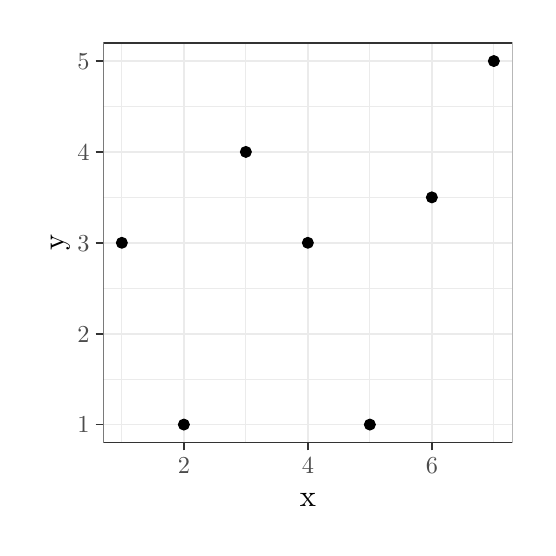
\begin{tikzpicture}[x=1pt,y=1pt]
\definecolor{fillColor}{RGB}{255,255,255}
\path[use as bounding box,fill=fillColor,fill opacity=0.00] (0,0) rectangle (180.67,180.67);
\begin{scope}
\path[clip] (  0.00,  0.00) rectangle (180.67,180.67);
\definecolor{drawColor}{RGB}{255,255,255}
\definecolor{fillColor}{RGB}{255,255,255}

\path[draw=drawColor,line width= 0.6pt,line join=round,line cap=round,fill=fillColor] (  0.00,  0.00) rectangle (180.68,180.68);
\end{scope}
\begin{scope}
\path[clip] ( 27.31, 30.69) rectangle (175.17,175.17);
\definecolor{fillColor}{RGB}{255,255,255}

\path[fill=fillColor] ( 27.31, 30.69) rectangle (175.17,175.17);
\definecolor{drawColor}{gray}{0.92}

\path[draw=drawColor,line width= 0.3pt,line join=round] ( 27.31, 53.67) --
	(175.17, 53.67);

\path[draw=drawColor,line width= 0.3pt,line join=round] ( 27.31, 86.51) --
	(175.17, 86.51);

\path[draw=drawColor,line width= 0.3pt,line join=round] ( 27.31,119.35) --
	(175.17,119.35);

\path[draw=drawColor,line width= 0.3pt,line join=round] ( 27.31,152.19) --
	(175.17,152.19);

\path[draw=drawColor,line width= 0.3pt,line join=round] ( 34.03, 30.69) --
	( 34.03,175.17);

\path[draw=drawColor,line width= 0.3pt,line join=round] ( 78.84, 30.69) --
	( 78.84,175.17);

\path[draw=drawColor,line width= 0.3pt,line join=round] (123.65, 30.69) --
	(123.65,175.17);

\path[draw=drawColor,line width= 0.3pt,line join=round] (168.45, 30.69) --
	(168.45,175.17);

\path[draw=drawColor,line width= 0.6pt,line join=round] ( 27.31, 37.25) --
	(175.17, 37.25);

\path[draw=drawColor,line width= 0.6pt,line join=round] ( 27.31, 70.09) --
	(175.17, 70.09);

\path[draw=drawColor,line width= 0.6pt,line join=round] ( 27.31,102.93) --
	(175.17,102.93);

\path[draw=drawColor,line width= 0.6pt,line join=round] ( 27.31,135.77) --
	(175.17,135.77);

\path[draw=drawColor,line width= 0.6pt,line join=round] ( 27.31,168.61) --
	(175.17,168.61);

\path[draw=drawColor,line width= 0.6pt,line join=round] ( 56.44, 30.69) --
	( 56.44,175.17);

\path[draw=drawColor,line width= 0.6pt,line join=round] (101.24, 30.69) --
	(101.24,175.17);

\path[draw=drawColor,line width= 0.6pt,line join=round] (146.05, 30.69) --
	(146.05,175.17);
\definecolor{drawColor}{RGB}{0,0,0}
\definecolor{fillColor}{RGB}{0,0,0}

\path[draw=drawColor,line width= 0.4pt,line join=round,line cap=round,fill=fillColor] ( 34.03,102.93) circle (  1.96);

\path[draw=drawColor,line width= 0.4pt,line join=round,line cap=round,fill=fillColor] ( 56.44, 37.25) circle (  1.96);

\path[draw=drawColor,line width= 0.4pt,line join=round,line cap=round,fill=fillColor] ( 78.84,135.77) circle (  1.96);

\path[draw=drawColor,line width= 0.4pt,line join=round,line cap=round,fill=fillColor] (101.24,102.93) circle (  1.96);

\path[draw=drawColor,line width= 0.4pt,line join=round,line cap=round,fill=fillColor] (123.65, 37.25) circle (  1.96);

\path[draw=drawColor,line width= 0.4pt,line join=round,line cap=round,fill=fillColor] (146.05,119.35) circle (  1.96);

\path[draw=drawColor,line width= 0.4pt,line join=round,line cap=round,fill=fillColor] (168.45,168.61) circle (  1.96);
\definecolor{drawColor}{gray}{0.20}

\path[draw=drawColor,line width= 0.6pt,line join=round,line cap=round] ( 27.31, 30.69) rectangle (175.17,175.17);
\end{scope}
\begin{scope}
\path[clip] (  0.00,  0.00) rectangle (180.67,180.67);
\definecolor{drawColor}{gray}{0.30}

\node[text=drawColor,anchor=base east,inner sep=0pt, outer sep=0pt, scale=  0.88] at ( 22.36, 34.22) {1};

\node[text=drawColor,anchor=base east,inner sep=0pt, outer sep=0pt, scale=  0.88] at ( 22.36, 67.06) {2};

\node[text=drawColor,anchor=base east,inner sep=0pt, outer sep=0pt, scale=  0.88] at ( 22.36, 99.90) {3};

\node[text=drawColor,anchor=base east,inner sep=0pt, outer sep=0pt, scale=  0.88] at ( 22.36,132.74) {4};

\node[text=drawColor,anchor=base east,inner sep=0pt, outer sep=0pt, scale=  0.88] at ( 22.36,165.58) {5};
\end{scope}
\begin{scope}
\path[clip] (  0.00,  0.00) rectangle (180.67,180.67);
\definecolor{drawColor}{gray}{0.20}

\path[draw=drawColor,line width= 0.6pt,line join=round] ( 24.56, 37.25) --
	( 27.31, 37.25);

\path[draw=drawColor,line width= 0.6pt,line join=round] ( 24.56, 70.09) --
	( 27.31, 70.09);

\path[draw=drawColor,line width= 0.6pt,line join=round] ( 24.56,102.93) --
	( 27.31,102.93);

\path[draw=drawColor,line width= 0.6pt,line join=round] ( 24.56,135.77) --
	( 27.31,135.77);

\path[draw=drawColor,line width= 0.6pt,line join=round] ( 24.56,168.61) --
	( 27.31,168.61);
\end{scope}
\begin{scope}
\path[clip] (  0.00,  0.00) rectangle (180.67,180.67);
\definecolor{drawColor}{gray}{0.20}

\path[draw=drawColor,line width= 0.6pt,line join=round] ( 56.44, 27.94) --
	( 56.44, 30.69);

\path[draw=drawColor,line width= 0.6pt,line join=round] (101.24, 27.94) --
	(101.24, 30.69);

\path[draw=drawColor,line width= 0.6pt,line join=round] (146.05, 27.94) --
	(146.05, 30.69);
\end{scope}
\begin{scope}
\path[clip] (  0.00,  0.00) rectangle (180.67,180.67);
\definecolor{drawColor}{gray}{0.30}

\node[text=drawColor,anchor=base,inner sep=0pt, outer sep=0pt, scale=  0.88] at ( 56.44, 19.68) {2};

\node[text=drawColor,anchor=base,inner sep=0pt, outer sep=0pt, scale=  0.88] at (101.24, 19.68) {4};

\node[text=drawColor,anchor=base,inner sep=0pt, outer sep=0pt, scale=  0.88] at (146.05, 19.68) {6};
\end{scope}
\begin{scope}
\path[clip] (  0.00,  0.00) rectangle (180.67,180.67);
\definecolor{drawColor}{RGB}{0,0,0}

\node[text=drawColor,anchor=base,inner sep=0pt, outer sep=0pt, scale=  1.10] at (101.24,  7.64) {x};
\end{scope}
\begin{scope}
\path[clip] (  0.00,  0.00) rectangle (180.67,180.67);
\definecolor{drawColor}{RGB}{0,0,0}

\node[text=drawColor,rotate= 90.00,anchor=base,inner sep=0pt, outer sep=0pt, scale=  1.10] at ( 13.08,102.93) {y};
\end{scope}
\end{tikzpicture}
